\documentclass[12pt,ignorenonframetext,]{beamer}
\setbeamertemplate{caption}[numbered]
\setbeamertemplate{caption label separator}{: }
\setbeamercolor{caption name}{fg=normal text.fg}
\beamertemplatenavigationsymbolsempty
\usepackage{lmodern}
\usepackage{amssymb,amsmath}
\usepackage{ifxetex,ifluatex}
\usepackage{fixltx2e} % provides \textsubscript
\ifnum 0\ifxetex 1\fi\ifluatex 1\fi=0 % if pdftex
  \usepackage[T1]{fontenc}
  \usepackage[utf8]{inputenc}
\else % if luatex or xelatex
  \ifxetex
    \usepackage{mathspec}
  \else
    \usepackage{fontspec}
  \fi
  \defaultfontfeatures{Ligatures=TeX,Scale=MatchLowercase}
\fi
\usetheme[]{Frankfurt}
\usecolortheme{lily}
% use upquote if available, for straight quotes in verbatim environments
\IfFileExists{upquote.sty}{\usepackage{upquote}}{}
% use microtype if available
\IfFileExists{microtype.sty}{%
\usepackage{microtype}
\UseMicrotypeSet[protrusion]{basicmath} % disable protrusion for tt fonts
}{}
\newif\ifbibliography
\hypersetup{
            pdftitle={Strategic Decision Making in the 3D Printing Industry},
            pdfauthor={Pedro Nascimento de Lima\^{}1, Maria Isabel Wolf Motta Morandi\^{}1, Daniel Pacheco Lacerda\^{}1},
            pdfborder={0 0 0},
            breaklinks=true}
\urlstyle{same}  % don't use monospace font for urls
\usepackage{longtable,booktabs}
\usepackage{caption}
% These lines are needed to make table captions work with longtable:
\makeatletter
\def\fnum@table{\tablename~\thetable}
\makeatother
\usepackage{graphicx,grffile}
\makeatletter
\def\maxwidth{\ifdim\Gin@nat@width>\linewidth\linewidth\else\Gin@nat@width\fi}
\def\maxheight{\ifdim\Gin@nat@height>\textheight0.8\textheight\else\Gin@nat@height\fi}
\makeatother
% Scale images if necessary, so that they will not overflow the page
% margins by default, and it is still possible to overwrite the defaults
% using explicit options in \includegraphics[width, height, ...]{}
\setkeys{Gin}{width=\maxwidth,height=\maxheight,keepaspectratio}

% Prevent slide breaks in the middle of a paragraph:
\widowpenalties 1 10000
\raggedbottom

\AtBeginPart{
  \let\insertpartnumber\relax
  \let\partname\relax
  \frame{\partpage}
}
\AtBeginSection{
  \ifbibliography
  \else
    \let\insertsectionnumber\relax
    \let\sectionname\relax
    \frame{\sectionpage}
  \fi
}
\AtBeginSubsection{
  \let\insertsubsectionnumber\relax
  \let\subsectionname\relax
  \frame{\subsectionpage}
}

\setlength{\parindent}{0pt}
\setlength{\parskip}{6pt plus 2pt minus 1pt}
\setlength{\emergencystretch}{3em}  % prevent overfull lines
\providecommand{\tightlist}{%
  \setlength{\itemsep}{0pt}\setlength{\parskip}{0pt}}
\setcounter{secnumdepth}{0}
\def\begincols{\begin{columns}}
\def\begincol{\begin{column}}
\def\endcol{\end{column}}
\def\endcols{\end{columns}}

\title{Strategic Decision Making in the 3D Printing Industry}
\subtitle{A Robust Decision Making (RDM) analysis}
\author{Pedro Nascimento de Lima\(^1\), Maria Isabel Wolf Motta Morandi\(^1\),
Daniel Pacheco Lacerda\(^1\)}
\institute{\(^1\) GMAP Research Group, UNISINOS University, RS, Brazil}
\date{November 14, 2018}

\begin{document}
\frame{\titlepage}

\section{Introduction}\label{introduction}

\begin{frame}{Motivation - DMDU and Business Decisions}

\begin{itemize}
\tightlist
\item
  Decision Makers in Business are faced with uncertainty, but\ldots{}
\item
  Testing quotation: (Lima 2018, Gong et al. (2017), Wholers (2016))
\end{itemize}

\end{frame}

\begin{frame}{Key Features of 3D printing}

\begin{itemize}
\tightlist
\item
  3D printing allows us to manufacture parts with unprecedented
  \textbf{complexity}, in \textbf{low volume};
\item
  By doing so, entire manufacturing industries might be disrupted by AM,
  presenting challenges to \ldots{}
\end{itemize}

\end{frame}

\begin{frame}{Two Column Layout}

\begincols
 \begincol{.48\textwidth}

\begin{itemize}
\tightlist
\item
  3D printing allows us to manufacture parts with unprecedented
  \textbf{complexity}, in \textbf{low volume};
\item
  By doing so, entire manufacturing industries might be disrupted by AM,
  presenting challenges to \ldots{}
\end{itemize}

\endcol
\begincol{.48\textwidth}

\includegraphics{dmdu-presentation_files/figure-beamer/test-1.pdf}

\endcol
\endcols

\end{frame}

\begin{frame}{Why 3D Printing?}

3D Printing is an emergint technology, but decision makers face
uncertainty.

\textbf{Positive Evidence}: - 3D printing Industry has seen two digits
growth consistently in the last few years; - 3D printing is already
reshaping supply chains across industries (e.g.: prothesis, aerospace,
etc.);

\textbf{Negative Evidence}: - Major players have been observing
declining profitability (e.g.: Stratasys, 3D Systems); - Estimates of 3D
printing growth diverge;

\end{frame}

\begin{frame}{Shaping events in the 3D Printing Industry}

\begin{itemize}
\tightlist
\item
  Patent Dynamics \& Patent Expiration (e.g.~FDM Patent);
\item
  Fierce Competition;
\item
  After the 3D printing Bubble, major players refocused their operations
  on industrial-grade printers;
\end{itemize}

\end{frame}

\section{XLRM}\label{xlrm}

\begin{frame}{Model Boundaries}

\begin{figure}
\centering
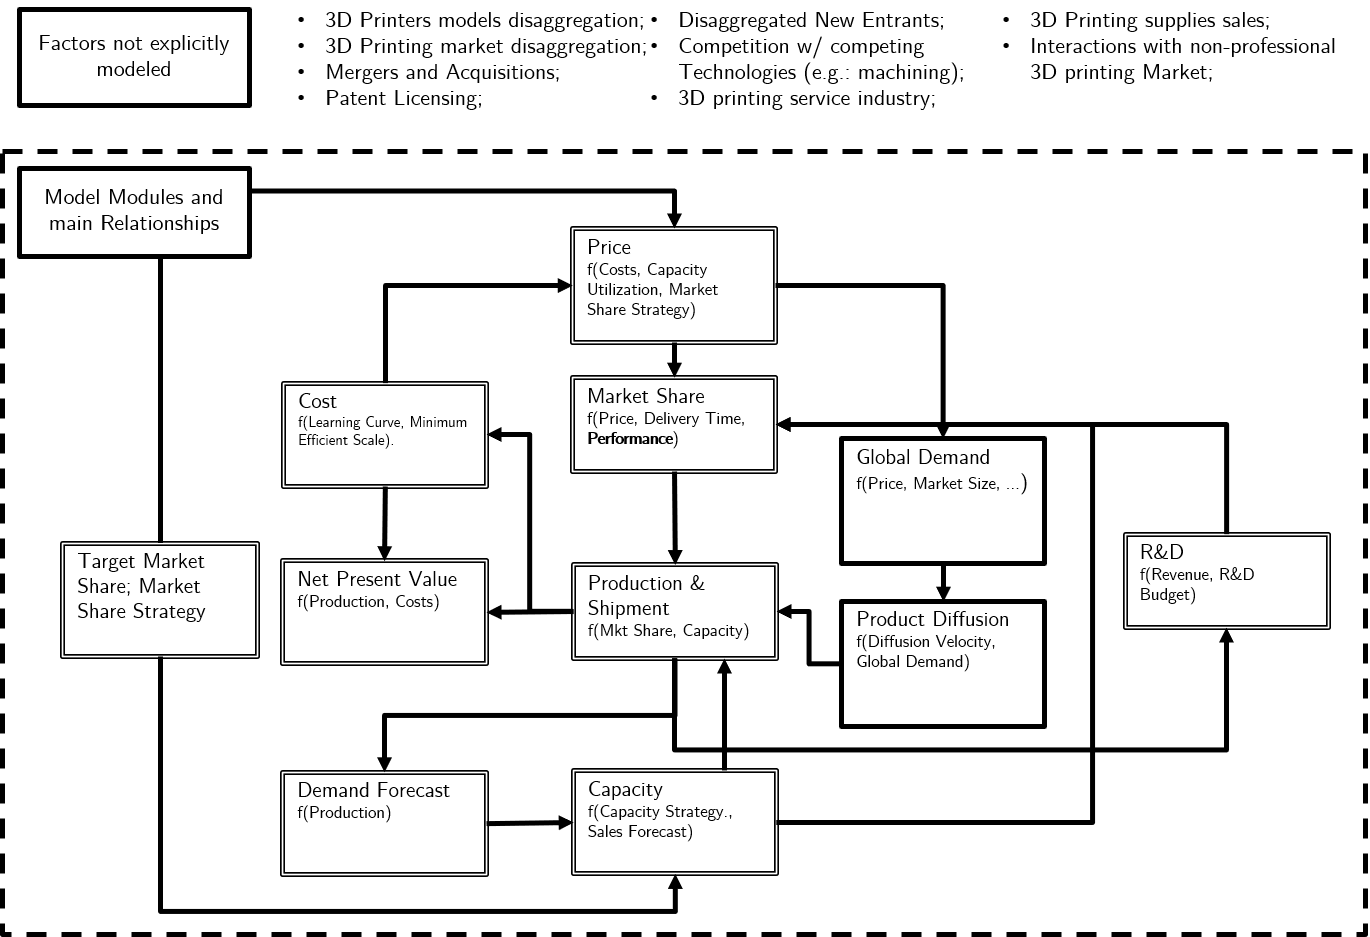
\includegraphics{images/model-modules-and-boundaries.png}
\caption{Model Structure \& Boundaries}
\end{figure}

\end{frame}

\section{Case Generation}\label{case-generation}

\begin{frame}{Design of Experiments}

\begin{itemize}
\tightlist
\item
  Full factorial design of these variables, resulting in 54 strategies:
\end{itemize}

\begin{longtable}[]{@{}lll@{}}
\toprule
\begin{minipage}[b]{0.14\columnwidth}\raggedright\strut
Variable\strut
\end{minipage} & \begin{minipage}[b]{0.47\columnwidth}\raggedright\strut
Meaning\strut
\end{minipage} & \begin{minipage}[b]{0.30\columnwidth}\raggedright\strut
Levels\strut
\end{minipage}\tabularnewline
\midrule
\endhead
\begin{minipage}[t]{0.14\columnwidth}\raggedright\strut
\(S_1\)\strut
\end{minipage} & \begin{minipage}[t]{0.47\columnwidth}\raggedright\strut
Market \& Pricing Strategy. Defines wether the player pursue an
agressive marketing strategy to gain market share (by cutting prices and
accepting excess capacity), or pursue a conservative strategy,\strut
\end{minipage} & \begin{minipage}[t]{0.30\columnwidth}\raggedright\strut
Agressive (1); Conservative (2)\strut
\end{minipage}\tabularnewline
\begin{minipage}[t]{0.14\columnwidth}\raggedright\strut
\(S_1^{max}\) or \(S_1^{min}\)\strut
\end{minipage} & \begin{minipage}[t]{0.47\columnwidth}\raggedright\strut
Desired Market Share. For a Conservative Strategy, the player adopts the
\(S_1^{max}\), and for an Agressive Strategy, \(S_1^{min}\)\strut
\end{minipage} & \begin{minipage}[t]{0.30\columnwidth}\raggedright\strut
20\%; 30\%; 40\%\strut
\end{minipage}\tabularnewline
\begin{minipage}[t]{0.14\columnwidth}\raggedright\strut
\(\eta_1\)\strut
\end{minipage} & \begin{minipage}[t]{0.47\columnwidth}\raggedright\strut
R \& D budget, as a fraction of revenue.\strut
\end{minipage} & \begin{minipage}[t]{0.30\columnwidth}\raggedright\strut
5\%; 10\%; 15\%\strut
\end{minipage}\tabularnewline
\begin{minipage}[t]{0.14\columnwidth}\raggedright\strut
\(\kappa_i\)\strut
\end{minipage} & \begin{minipage}[t]{0.47\columnwidth}\raggedright\strut
Fraction of R \& D budget released to open source technologies.\strut
\end{minipage} & \begin{minipage}[t]{0.30\columnwidth}\raggedright\strut
0 \%; 50 \%; 90 \%\strut
\end{minipage}\tabularnewline
\bottomrule
\end{longtable}

\end{frame}

\begin{frame}{Candidate Strategy NPV across scenarios}

\begin{center}\includegraphics{dmdu-presentation_files/figure-beamer/unnamed-chunk-1-1} \end{center}

\end{frame}

\begin{frame}{Global Demand across scenarios}

\begin{center}\includegraphics{dmdu-presentation_files/figure-beamer/unnamed-chunk-2-1} \end{center}

\end{frame}

\begin{frame}{4 Players Net Present Value in a given scenario}

\begin{center}\includegraphics{dmdu-presentation_files/figure-beamer/unnamed-chunk-3-1} \end{center}

\end{frame}

\begin{frame}{Net Present Value across strategies and Scenarios}

\begin{center}\includegraphics{dmdu-presentation_files/figure-beamer/unnamed-chunk-4-1} \end{center}

\end{frame}

\begin{frame}{Regret across strategies and Scenarios}

\begin{center}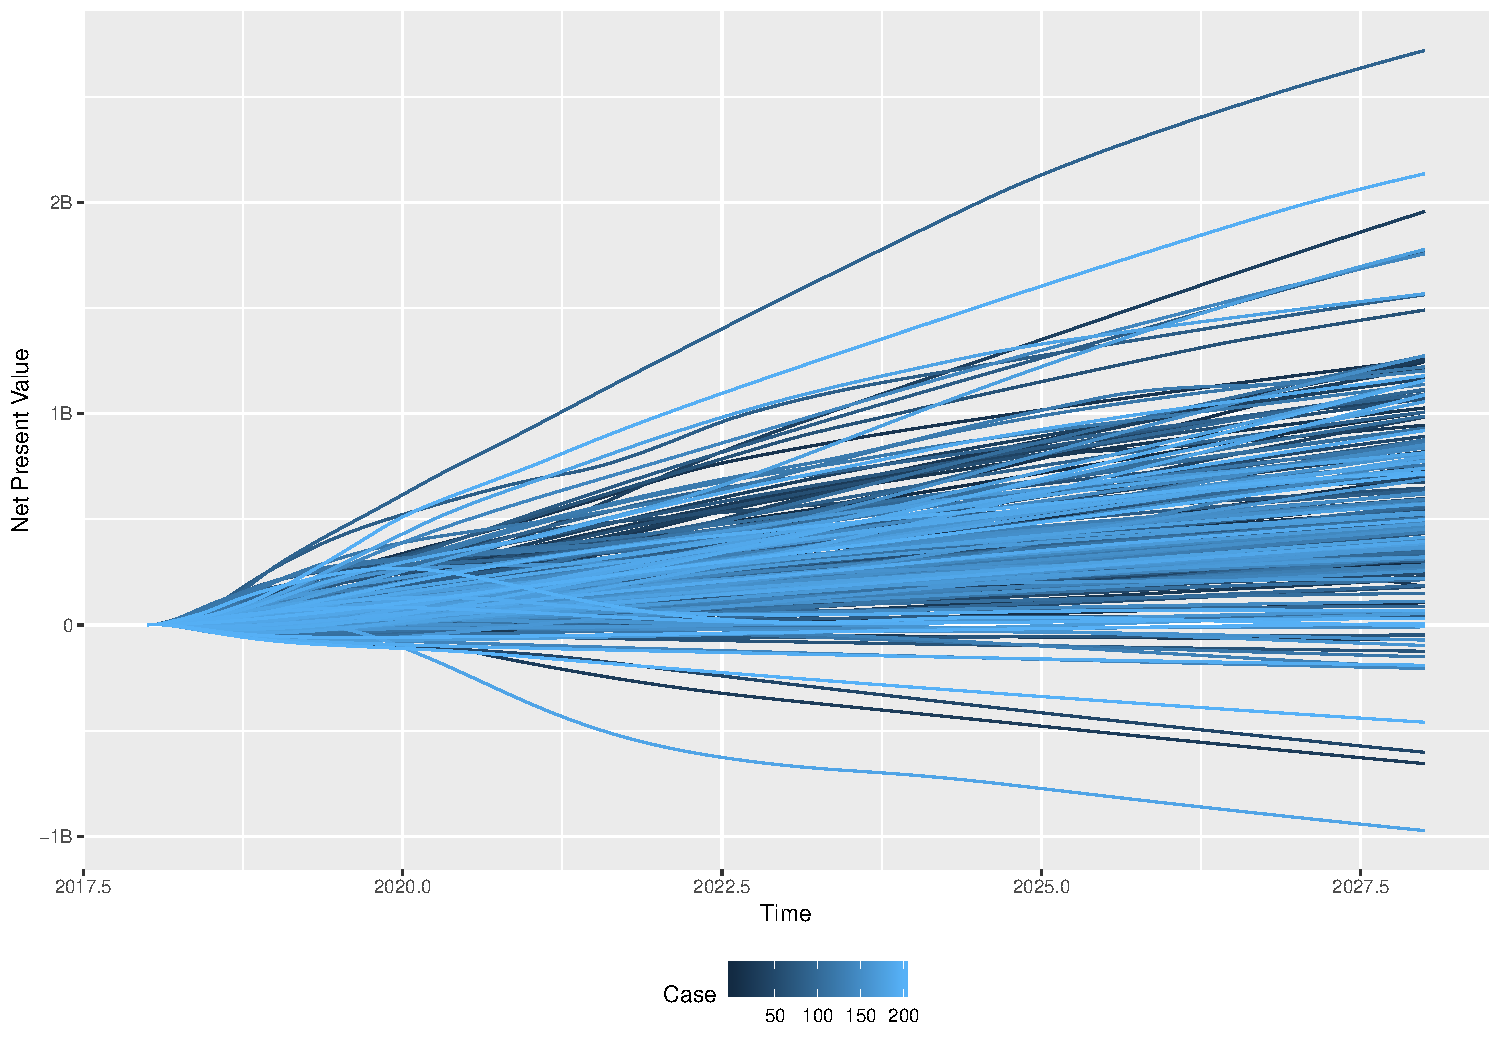
\includegraphics{dmdu-presentation_files/figure-beamer/unnamed-chunk-5-1} \end{center}

\end{frame}

\begin{frame}{Ranking Strategies by Regret}

\end{frame}

\section{Scenario Discovery}\label{scenario-discovery}

\section*{Conclusions}\label{conclusions}
\addcontentsline{toc}{section}{Conclusions}

\hypertarget{refs}{}
\hypertarget{ref-Gong2017}{}
Gong, Min, Robert Lempert, Andrew Parker, Lauren A. Mayer, Jordan
Fischbach, Matthew Sisco, Zhimin Mao, David H. Krantz, and Howard
Kunreuther. 2017. ``Testing the scenario hypothesis: An experimental
comparison of scenarios and forecasts for decision support in a complex
decision environment.'' \emph{Environmental Modelling \& Software} 91.
Elsevier Ltd: 135--55.
doi:\href{https://doi.org/10.1016/j.envsoft.2017.02.002}{10.1016/j.envsoft.2017.02.002}.

\hypertarget{ref-Lima2018}{}
Lima, Pedro Nascimento de. 2018. ``Avaliação de Decisões Estratégicas
sob Incerteza Profunda na Indústria da Manufatura Aditiva: Uma Análise a
partir do método Robust Decision Making (RDM).'' Masters Dissertation,
UNISINOS.
\url{http://www.repositorio.jesuita.org.br/handle/UNISINOS/6991}.

\hypertarget{ref-Wholers2016}{}
Wholers, Terry. 2016. ``Popularity of FDM.''
\url{https://wohlersassociates.com/blog/2016/01/popularity-of-fdm/}.

\end{document}
